%\documentclass[english]{beamer}
\documentclass[english,hangout]{beamer}
%\documentclass[aspectratio=169]{beamer}
%\usepackage{amsmath}
%\usepackage{amssymb}
\usepackage{rotating}
\usepackage{verbatim}
\usepackage{latexsym}
\usepackage{graphicx}
\usepackage{tabularx}
\usepackage{ragged2e}
\usepackage{eurosym}   % Euro symbol: \euro
\usepackage{listings}
\usepackage{multirow}
\usepackage{colortbl}
\usepackage{textcomp}  % many special symbols
\usepackage{lmodern}
\usepackage{times}
\usepackage[T1]{fontenc}
\usepackage[utf8]{inputenc}
\usepackage[english]{babel}
\usepackage{booktabs}

\graphicspath{{./images/Beamer/}}

\usetheme[fb2]{FrankfurtUniversity}
%\usetheme[fb2,noslogan]{FrankfurtUniversity}
%\slogan{\large\color{red}UNAUTHORIZED}


\title{Explainable SVM}
\subtitle{Digitalization Project "Webtools for teaching"}
\author{H. Pfaff, L. Atkinson, L. Jordan \& Y. Er}
\institute{Frankfurt University of Applied Sciences\\
           Faculty of Computer Science and Engineering\\}
\date{10.09.2020}%{\today}%{January 15, 2015}


\begin{document}

% Notes:
%
% * Introduction: why this topic is so important, why web visualzations are
%   important (Corona!)
% * SVM at high level (1 SLIDE !!!)
% * split up SVM visualization part
% * used technologies (1 slide)
% * implementation of SVM in JS (1 slide)
% * live demo
%   * available controls & features (see user manual in doc)
%   * step through explanation tabs
% * Challenges
%   * 1 slide: d3 vs plotly
%   * 1 slide: svm implementation, testing, debugging
%   * 1 slide: generating data sets with Python
%   * 1 slide: plotting challenges (sigmoid smoothing, countours vs drawing a line)
% * Future work, conclusion (1 slide)
% * Questions, references (1 slide)

% Screenshots:
% * diagram with/without smoothing (edit plotly_gui.js to use signum instead of sigmoid)
% * used technologies: logos?
% * generating data sets: plots of salmon vs iris

\begin{frame}
	\titlepage
\end{frame}

\begin{frame}
	\frametitle{Agenda}
	\tableofcontents[hideallsubsections]
\end{frame}
%\addtocounter{framenumber}{-1}

\section{Introduction}
\begin{frame}
	\frametitle{Introduction}

  \begin{itemize}
  \item SVMs important machine learning algorithm
  \item support web-based teaching via interactive visualizations
  \item distance learning more important due to Corona
  \end{itemize}
  % TODO: stock image of home office like something?
\end{frame}

\section{Support Vector Machines}
\begin{frame}
	\frametitle{SVM}

  \begin{itemize}
  \item supervised learning
  \item commonly used for classification, also regression
  \item learning means finding a separating boundary (hyperplane)
  \item Vapnik \& Chervonenkins 1963
  \end{itemize}
\end{frame}

% 	\framesubtitle{plotly.js vs. d3.js}
	
% 	\begin{itemize}
% 		\item \textbf{\textit{d3.js}}
% 		\begin{itemize}
% 			\item d3.js offers great individuality for all kinds of data visualizations and user interfaces
% 			\item surplus of possibilities requires intensive incorporation
% 			\item simple visualization like \textit{line, scatter} or \textit{contour} plots tend to be more difficult
% 		\end{itemize}
% 		\item \textbf{\textit{plotly.js}}
% 		\begin{itemize}
% 			\item previous knowledge through R and Python
% 			\item specialized on visualizations of data, models and statistics
% 			\item standardized pipelines for common types of plots
% 			\item highly customizable through simple commands

% 		\end{itemize}
% 	\end{itemize}
% \end{frame}

% \begin{frame}
% 	\frametitle{SVM Visualization}
% 	\framesubtitle{Major Components}
% 	\begin{itemize}
% 		\item Contour Plot
% 		\begin{itemize}
% 			\item drawing of the decision boundaries 
% 			\item two vectors are filled with values between $\min()$ and $\max()$ of  both features
% 			\item for drawing the boundaries, the SVM predicts all combinations of these two features $\rightarrow$ array of predictions $\textbf{Z}$
% 			\item through $\textbf{Z}$ and a smoothing function, such as \textit{Sigmoid}, a heatmap can be drawn that visualizes the decision boundaries of the SVM
% 		\end{itemize}

% 		\item Scatter Plot
% 		\begin{itemize}
% 			\item Support Vectors
% 			\item Data Points
% 		\end{itemize}
% 	\end{itemize}
% \end{frame}

% \begin{frame}
% 	\frametitle{The Z-Array}
% 	\begin{figure}
% 		\centering
% 		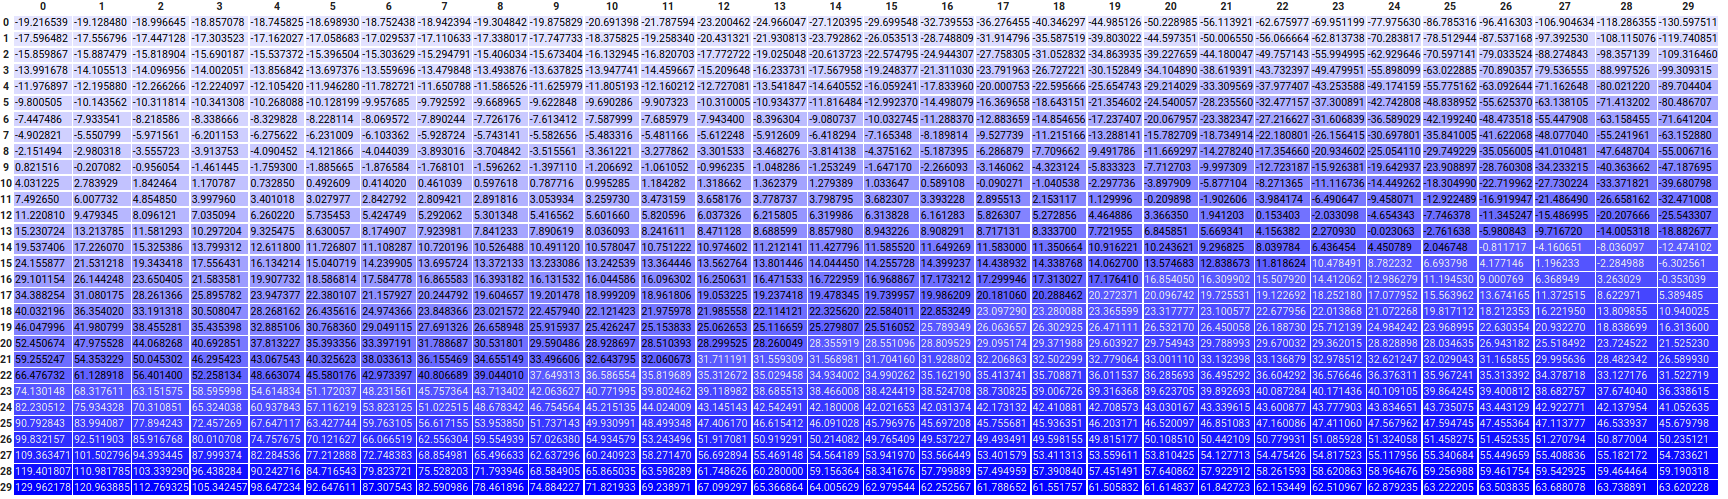
\includegraphics[width=11cm]{Z-Array.png}
% 	\end{figure}
% 	\begin{itemize}
% 		\item Decision boundary may be drawn between positive and negative values
% 		\item Using \textit{sign} or \textit{Sigmoid} the decision boundary can be displayed in a contour plot as a clear and smoothed line
% 	\end{itemize}
% \end{frame}

% \begin{frame}
% 	\frametitle{Final Plot}
% 	\begin{figure}
% 		\centering
% 		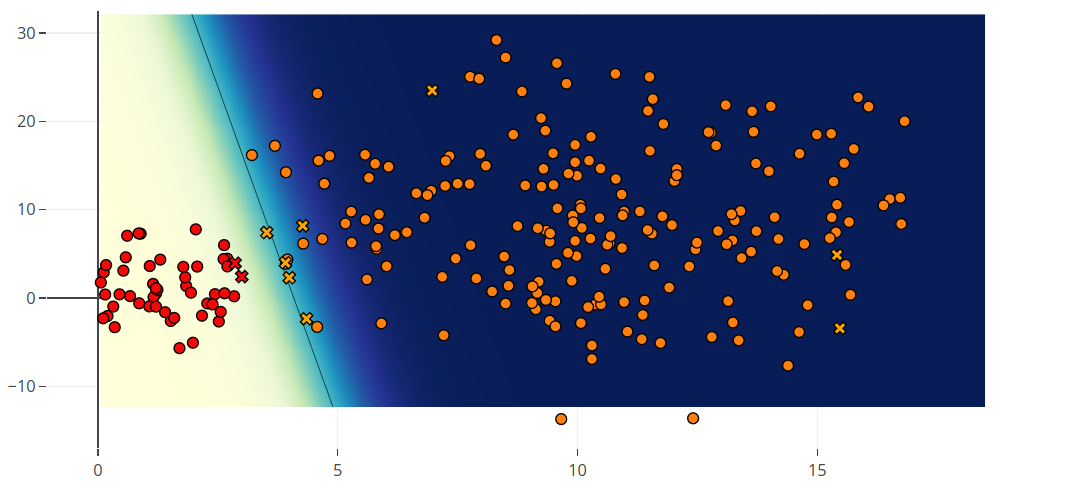
\includegraphics[width=11cm]{FinalPlot.png}
% 	\end{figure}
% 	\begin{itemize}
% 		\item Final result of the combination of scatter and contour plots
% 		\item Support vectors are shown as X's
% 		\item Class memberships are displayed through differing colors
% 	\end{itemize}
% \end{frame}

\section{Used Technologies}
\begin{frame}
	\frametitle{Used Technologies}
	% TODO: logos of technologies
  % TODO: logo: HTML5
  % TODO: logo: css
  % TODO: logo: bootstrap
  % TODO: logo: jquery
  % TODO: logo: mathjax
  % TODO: logo: plotly
\end{frame}

\section{Live Demo}
\begin{frame}[plain]
	\begin{center}
		\textbf{Live Demo}
	\end{center}
\end{frame}

\section{Solved Challenges}
% * 1 slide: d3 vs plotly
% * 1 slide: svm implementation, testing, debugging
% * 1 slide: generating data sets with Python
% * 1 slide: plotting challenges (sigmoid smoothing, countours vs drawing a line)

\begin{frame}
	\frametitle{Solved Challenges: D3 vs Plotly}

  \begin{itemize}
  \item d3 is very flexible
  \item d3 is very low-level, SVG-oriented
  \item Plotly has standard pipelines for common plot types
  \item Plotly is still very customizable (builds upon d3)
  \end{itemize}

\end{frame}

\begin{frame}[fragile]
	\frametitle{Solved Challenges: SVM Implementation}
  Implemented API:
  \begin{itemize}
  \item \verb|svm = new SVM({ X, y, C, tol, kernel })|
    \begin{itemize}
    \item \verb|kernel| can be any function \verb|(x, y) -> float|
    \end{itemize}
  \item \verb|classification = svm.output(point)|
  \item \verb|svm.main_routine()|
  \item \verb|svm.main_routine_step({examine_all})|
  \end{itemize}
\end{frame}

\begin{frame}
	\frametitle{Solved Challenges: Data Sets}
  % TODO: plots with iris, salmon

  implemented Python script to generate new data sets
\end{frame}

\begin{frame}
	\frametitle{Solved Challenges: Plotting}
  % * 1 slide: plotting challenges (sigmoid smoothing, countours vs drawing a line)
  % TODO: picture of plot without smoothing
  \begin{itemize}
  \item smoothing
    \begin{itemize}
    \item use sigmoid function instead of sign
    \end{itemize}
  \item drawing the separating boundary
    \begin{itemize}
    \item drawing a line doesn't work for all kernels
    \item calculating line equation is difficult
    \item simple trick: use a 2-level contour plot
    \end{itemize}
  \end{itemize}
\end{frame}


\section{Conclusion}
\begin{frame}
	\frametitle{Conclusion}

  \begin{itemize}
  \item built a wonderful SVM visualization
  \item great teamwork, complementary skills
  \item future work
    \begin{itemize}
    \item step through SVM convergence
    \item drawing margins around the hyperplane
    \item more kernel functions
    \end{itemize}
  \end{itemize}
  
\end{frame}

\begin{frame}[plain]
	\begin{center}
		\textbf{Any Questions?}
	\end{center}
\end{frame}

\begin{frame}
	\frametitle{References}
	
\end{frame}


%\section{Normal Slide}
%
%\begin{frame}[fragile]
% \frametitle{Example of Normal Slide}
% \framesubtitle{Subtitle}
% Lorem ipsum dolor sit amet, consectetur adipiscing elit. Etiam sit amet
% vulputate ante, vel laoreet erat. Cras pulvinar, sem nec lobortis vehicula,
% leo dolor commodo.
% 
%  \begin{itemize}
%   \item Item 1
%   \item Item 2:
%     \begin{itemize}
%      \item Subitem 2.1
%      \item\dots
%     \end{itemize}
%  \end{itemize}
%\end{frame}
%
%
%
%\section{Floats}
%
%\subsection{Figures}
%
%\begin{frame}
%\frametitle{Figure on slide}
%\begin{center}
%%\includegraphics[height=7.5cm]{shall_i_give_him_a_hint.png}
%\end{center}
%\vspace{-6mm}
%\tiny Artist: Tony Auth
%\end{frame}
%
%
%
%\begin{frame}
%\frametitle{Image and Bullet Points Side by Side}
%\begin{columns}[onlytextwidth]
%\begin{column}{.7\textwidth}
%\begin{itemize}
%\item \textbf{Lorem ipsum} 
%\begin{enumerate}
%\item Lorem ipsum dolor sit amet, consectetur adipiscing elit.
%\item Donec ut est laoreet, sagittis tortor ac, rhoncus metus.
%\end{enumerate}
%\item \textbf{Etiam eget} 
%\begin{itemize}
%\item Etiam eget lectus ac nisl blandit pretium in id velit.
%\end{itemize}
%\end{itemize}
%\end{column}
%
%\begin{column}{.3\textwidth}
%%\includegraphics[width=\textwidth]{me}
%\end{column}
%\end{columns}
%
%\vspace{-.7mm}
%\begin{itemize}
%\item \textbf{Ut in lorem sollicitudin}
%\begin{itemize}
%\item Ut in lorem sollicitudin, condimentum magna ac, condimentum urna.
%\item Ut malesuada eros id odio rutrum auctor varius a mi.
%\item Nulla nec sapien condimentum, faucibus libero at, tristique ante.
%\end{itemize}
%\end{itemize}
%\end{frame}
%
%
%
%\subsection{Tables}
%
%\begin{frame}
% \frametitle{Example of a Table}
%\begin{table}[ht]
% \begin{tabular}{clrr} \toprule
% 2015 (2014)	& 	Language 	& Ratings 	& Change \\
% \midrule
%1	(1)		& C		& 16.703\%	& -1.24\% \\
%2	   (2)		& Java	& 15.528\%	& -1.00\% \\
%3	   (3)		& Objective-C	& 6.953\%	& -4.14\% \\
%4	   (4)		& C++	& 6.705\%	& -0.86\% \\
%5	   (5)		& C\#		& 5.045\%	& -0.80\% \\
%6	   (6)		& PHP	& 3.784\%	& -0.82\% \\
%7	   (9)		& JavaScript	& 3.274\%	& \emph{+1.70\%} \\
%8	   (8)		& Python	& 2.613\%	& +0.24\% \\
%9	 (13)		& Perl	& 2.256\%	& +1.33\% \\
%10	 (17)		& PL/SQL	& 2.014\%	& +1.38\% \\
%\bottomrule
% \end{tabular}
% \caption{TIOBE Index as of January 2015}
%\end{table}
%\vspace{-3mm}
%\tiny Source: \texttt{http://www.tiobe.com}
%\end{frame}
%
%
%
%\section{Emphasize}
%
%\subsection{Block}
%
%\begin{frame}
% \frametitle{Using the \texttt{block} environment}
%\begin{block}{Title of Bock}
%  Content of block goes here.
%\end{block}
%
%\begin{exampleblock}{Example No. 42}
%  This is an example.
%\end{exampleblock}
% 
%\begin{alertblock}{Watch out!!!}
%  You must not do that!
%\end{alertblock}
%\end{frame}
%
%
%
%\subsection{Text Emphasize}
%
%\begin{frame}
% \frametitle{Using the \texttt{\textbackslash emph} command}
%You can \emph{emphasize} words by using \texttt{\textbackslash emph\{emphasize\}}.
%
%It will automatically use the color of your faculty.
%
%\vspace{\baselineskip}
%BTW you can access all the different colors as \texttt{FB1Color}, \texttt{FB2Color} etc.
%\end{frame}
%
%
%
%\subsection{Code Blocks}
%
%\begin{frame}[fragile]
% \frametitle{Displaying chunks of code}
%
%\begin{lstlisting}[language=Python]
%part = new Part()
%part.name = "Sample part"
%part.price = 123.45
%part.save()
%\end{lstlisting}
%
%Another example with \blank{SQL}:
%
%\begin{lstlisting}[language=sql]
%INSERT INTO parts (name, price) VALUES ('Sample part', 123.45);
%\end{lstlisting}
%
%\begin{alertblock}{You must not forget}
%  \dots\ to mark your frame as \texttt{[fragile]}
%\end{alertblock}
%\end{frame}



\end{document}